\documentclass[11pt,a4paper,leqno]{report}
\usepackage{tikz}
%\usepackage[german]{babel}
\usepackage{amsmath}
\usepackage{amsthm}
\usepackage{amssymb}
\usepackage{float}
\usepackage{amsfonts}
\usepackage{hyperref}
\usepackage{lmodern}
%\usepackage{makeidx}
%\usepackage{graphicx}
%\graphicspath{{pics/}}
\usepackage{svg}
\usepackage{amsmath}
\usepackage{delarray}
\makeatletter
\renewcommand*\env@matrix[1][*\c@MaxMatrixCols c]{%
	\hskip -\arraycolsep
	\let\@ifnextchar\new@ifnextchar
	\array{#1}}
\makeatother
\newcommand{\eps}{\varepsilon}
\newcommand{\R}{\mathbb{R}}
\newcommand{\C}{\mathbb{C}}


%%%%%%%%%%% REST %%%%%%%%%%%%%%%%%%%%%%%%%%%%%%%%%%%%

\DeclareMathOperator{\dom}{dom}
\DeclareMathOperator{\ran}{ran}
\newcommand{\re}{\mathrm{Re}}
\newcommand{\im}{\mathrm{Im}}

\newcommand{\ul}{\underline}
\newcommand{\I}{\mathrm{i}}
\newcommand{\E}{\mathrm{e}}

%\makeindex
%\setlength{\parindent}{0em} 


\newtheorem{theorem}{Theorem}[chapter]
\newtheorem{proposition}{Satz}[chapter]
\newtheorem{lemma}[theorem]{Lemma}
\newtheorem{definition}[theorem]{Definition}
\newtheorem{corollary}[theorem]{Folgerung}
\newtheorem{remark}[theorem]{Bemerkung}

\renewcommand{\figurename}{Abbildung}
\numberwithin{equation}{chapter}



\usepackage{listings}
\lstset{basicstyle=\ttfamily}
\lstset{literate=%
	{\"o}{{\"O}}1
	{\"a}{{\"A}}1
	{\"u}{{\"U}}1
	{\"u}{{\"u}}1
	{\"a}{{\"a}}1
	{\"o}{{\"o}}1
}
\renewcommand{\chaptername}{Kapitel}
\renewcommand{\contentsname}{Inhaltsverzeichnis}
\renewcommand{\proofname}{Beweis}
\begin{document}


\begin{titlepage}

\vspace*{5cm}
\begin{center}
\rule{\linewidth}{0.5mm} \\[0.4cm]
{ \Huge \bfseries Graphische elektronische Methoden} \\[0.2cm]
\rule{\linewidth}{0.5mm} \\[3.5cm]
\begin{minipage}[t]{0.4\textwidth}
\begin{flushleft} \large
\emph{Author:}\\
Oliver \textsc{Sko\v{c}ek} \\[4cm]
\small

\end{flushleft}

\end{minipage}
\begin{minipage}[t]{0.4\textwidth}

\end{minipage}
 
% Bottom of the page

 
\end{center}
 
\end{titlepage}

%\maketitle


%\renewcommand{\contentsname}{Contents}

\tableofcontents

\markboth{Contents}{Contents}

\vfill


\chapter*{Einf\"uhrung}
Es werden einige Grundlagen der Graphentheorie eingef\"uhrt. Insbesondere werden planare Graphen und die zugeh\"orenden dualen Graphen definiert. Anschließend werden Funktionenr\"aume auf Graphen definiert und zum Gradienten, der Divergenz und der Rotation aus der Vektoranalysis analoge Operatoren, die jene R\"aume ineinander \"uberf\"uhren. Ein zum de Rham Komplex analoges Theorem wird vorgestellt und bewiesen. Die so entwickelte Theorie wird anschlie\ss{}end verwendet um das verallgemeinerte Poissonproblem und seine L\"osungstheorie zu formulieren. Abschließend wird analog zu den zweidimensionalen Maxwellgleichungen, ein gew\"ohnliches lineares Differentialgleichungssystem vorgestellt und dessen L\"osbarkeit untersucht.

\chapter{Planare Graphen}

	Ein Graph besteht aus Ecken $V$ und Kanten $E$. Die Ecken und Kanten stehen in Beziehung zueinander. Man sagt eine Kante \emph{verbindet} zwei Ecken. Wir wollen nur solche Graphen betrachten, deren Kanten jeweils zwei unterschiedliche Ecken verbinden.
\begin{figure}[H]
	\begin{center}
		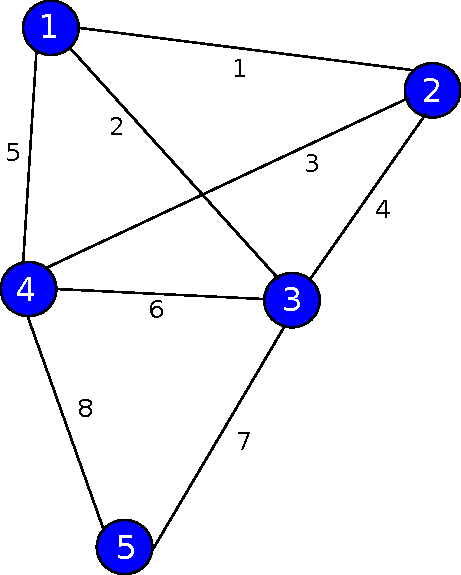
\includegraphics[scale=0.4]{Abbildungen/graph_1.pdf}
		\caption{Beispiel Graph.}
	\end{center}
\end{figure}
\noindent
	Die Beziehung zwischen Ecken und Kanten kann durch eine Matrix dargestellt werden. Der vertikale Index der Matrix steht f\"ur die Kanten und der horizontale Index steht f\"ur die Ecken. Die Matrix ist Eins falls die Kante die Ecke mit einer anderen Ecke verbindet und sonst Null. Diese Matrix nennt man die \textbf{Inzidenzmatrix} des Graphen.\\
	Als Beispiel betrachte die Inzidenzmatrix des Graphen in Abbildung 2.1.
	\begin{center}
		\begin{tabular}{c c c c c}
			1 & 1 & 0 & 0 & 0\\
			1 & 0 & 1 & 0 & 0\\
			0 & 1 & 0 & 1 & 0\\
			0 & 1 & 1 & 0 & 0\\
			1 & 0 & 0 & 1 & 0\\
			0 & 0 & 1 & 1 & 0\\
			0 & 0 & 1 & 0 & 1\\
			0 & 0 & 0 & 1 & 1\\
		\end{tabular} 
	\end{center}
	Im Grunde interessieren wir uns nicht f\"ur die spezielle Realisierung von Ecken und Kanten, sondern f\"ur die Verbindungsstruktur, die genau durch die Inzidenzmatrix festgelegt wird. Dies legt folgende Definition nahe.
\begin{definition}
	Ein \textbf{Graph} ist eine Matrix (Inzidenzmatrix) deren Zeilensumme zwei ist. Zwei Graphen mit Inzidenzmatrizen $X$ und $Y$ sind gleich falls man $X$ aus $Y$ durch Vertauschung von Zeilen und Spalten erhalten kann.
\end{definition}
\begin{remark}
	Alternativ kann ein Graph auch durch eine Adjazenzmatrix definiert werden. Eine solche Matrix ist quadratisch und beide Indizes stehen f\"ur die Ecken des Graphen. Die Adjazenzmatrix ist eins falls die Ecken durch eine Kante verbunden sind und sonst Null. Als Beispiel die Adjazenzmatrix unseres Beispielgraphen.
	\begin{center}
	\begin{tabular}{c c c c c}
		0 & 1 & 1 & 1 & 0\\
		1 & 0 & 1 & 1 & 0\\
		1 & 1 & 0 & 1 & 1\\
		1 & 1 & 1 & 0 & 1\\
		0 & 0 & 1 & 1 & 0\\
	\end{tabular} 
\end{center}
	Der Nachteil der Adjazenzmatrix ist, dass sie keine Mehrfachkanten zwischen zwei Ecken zul\"asst.
\end{remark}
\noindent
Manchmal ist es notwendig \"uber Teile von Graphen zu sprechen. Hierzu dient das Konzept des Teilgraphen. Ein Teilgraph eines Graphen $G$ ist ein Graph, den man durch entfernen von Ecken und Kanten aus $G$ erh\"alt. Bedenke dabei, dass mit jeder Ecke auch alle diese Ecke verbindenten Kanten entfernt werden m\"ussen.
\begin{definition}
	Sei $G$ ein Graph mit Inzidenzmatrix $X$ und $H$ ein Graph mit Inzidenzmatrix $Y$, dann ist $G$ ein \textbf{Teilgraph} von $H$, falls man die Matrix $X$ durch entfernen von Zeilen oder Spalten aus der Matrix $Y$ erhalten kann.
\end{definition}
\noindent
Betrachten wir hierzu einen Teilgraph des Beispielgraphen.
\begin{figure}[H]
	\begin{center}
		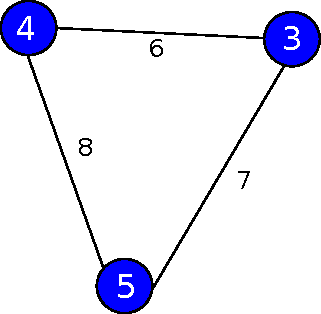
\includegraphics[scale=0.4]{Abbildungen/graph_1_teil.pdf}
		\caption{Teilgraph des Beispielgraphs.}
	\end{center}
\end{figure}
\noindent
Die zugeh\"orige Inzidenzmatrix erhalten wir indem wir die ersten beiden Spalten entfernen und anschlie{\ss}end alle Zeilen, deren Summe ungleich zwei ist. 
\noindent
Das Resultat ergibt dann f\"ur kannten 4, 7 und 8 folgende Inzidenz mit den Ecken 3, 4 und 5.
	\begin{center}
	\begin{tabular}{c c c}
		1 & 1 & 0\\
		1 & 0 & 1\\
		0 & 1 & 1\\
	\end{tabular} 
\end{center}
Eine spezielle Art von Teilgraph erh\"alt man, wenn man eine Teilmenge $U$ der Ecken fixiert und alle Kanten aus dem Graphen entfernt, die eine nicht in der Teilmenge $U$ enthaltene Ecke verbinden. Man nennt so einen Graph den durch die Menge $U$ \textbf{induzierten Teilgraph}. Der Teilgraph in Abbildung 2.2 ist ein solches Beispiel. Es ist der durch $U =\{3, 4, 5\}$ induzierte Teilgraph des Beispielgraphen.
\begin{definition}
	Sei $G$ ein Graph, dann nennt man $G$ \textbf{zusammenh\"angend} falls man von jeder Ecke von $G$ jede andere Ecke \"uber Kanten erreichen kann. Sei weiters $k\in\mathbb{N}$, dann sagt man ein Graph ist \textbf{$k$-fach zusammen\-h\"angend}, falls man $k - 1$ beliebige Kanten entfernen k\"onnte und der resultierende Graph immer noch zusammenh\"angend w\"are.
\end{definition}
\noindent
Alle Graphen werden von hier an als zusammenh\"angend angenommen. Allgemein l\"asst sich jeder Graph als Ansammlung von zusammenh\"angenden Teilgraphen darstellen, wodurch diese Annahme im Sinne einer Vereinfachung gerechtfertigt wird.
\begin{definition}
	Ein Graph hat eine \textbf{planare Darstellung} wenn man den Graph auf einem Blatt Papier zeichnen kann, indem man f\"ur jede Ecke einen Punkt zeichnet und f\"ur jede Kante einen Strich zwischen den Eck-Punkten, die sie verbinden soll, ohne das sich dabei zwei Striche kreuzen.
\end{definition}
\noindent
	Der Graph aus Abbildung 2.1 hat eine planare Darstellung. Um dies zu sehen muss man nur die Position von Ecke Nummer 2 ver\"andern.
\begin{figure}[H]
	\begin{center}
		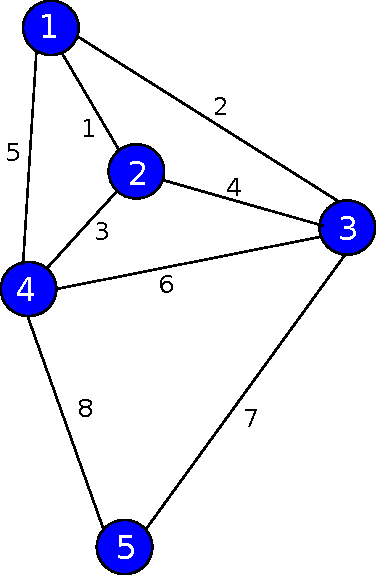
\includegraphics[scale=0.4]{Abbildungen/graph_1_planar.pdf}
		\caption{Beispiel Graph (planar).}
	\end{center}
\end{figure}
\noindent
	Im Allgemeinen gibt es mehrere Wege wie ein bestimmter Graph gezeichnet werden kann. Es gibt sogar f\"ur ein und denselben Graphen oft mehrere planare Darstellungen.
\begin{figure}[H]
	\begin{center}
		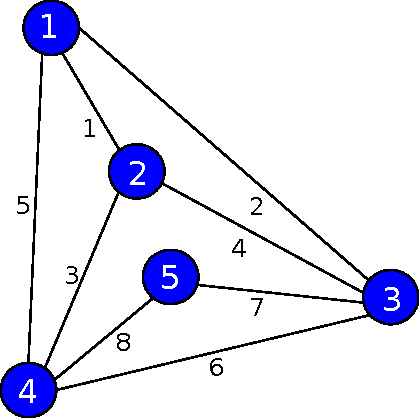
\includegraphics[scale=0.4]{Abbildungen/graph_1_planar2.pdf}
		\caption{Beispiel Graph (planar) alternativ.}
	\end{center}
\end{figure}
\noindent
Es ist also zus\"atzliche Information notwendig um eine planare Darstellung eindeutig festzulegen. Diese zus\"atzliche Information kann \"uber die Fl\"achen aus denen sich die planare Darstellung zusammensetzt gegeben werden.\\
\begin{definition}
	Sei $G$ ein Graph, dann nennt man $G$ einen \textbf{Zyklus} oder \textbf{zyklisch}, falls jede Ecke von $G$ mit genau zwei Kanten verbunden ist.
\end{definition}
\noindent
Betrachten wir eine der planaren Darstellungen des Beispielgraphen. Eine \textbf{Fl\"ache} ist hier ein Zyklus, der keine Ecke einschlie\ss{}t.
\begin{remark}
	Sei $G$ ein Graph und $\{A_1, A_2, \dots, A_n\}$ eine Menge von zyklischen induzierten Teilgraphen, sodass jede Kante von $G$ in maximal zwei der Zyklen vorkommt und jede Ecke von $G$ in mindestens einem der Zyklen vorkommt, dann gibt es eine eindeutige planare Darstellung des Graphen $G$, dessen Fl\"achen genau die $\{A_1, A_2, \dots, A_n\}$ sind.  
\end{remark}
\begin{definition}
	Ein planarer Graph $G=(g, f)$ ist ein Graph $g$ und eine Menge $f$ von Zyklen aus $g$ wie in Bemerkung 1.6. beschrieben. Sei weiters $e$ eine Kante von $g$, dann sagt man $e$ liegt am \textbf{Rand} des Graphen wenn $e$ genau einmal in einer Fl\"ache vorkommt. Der Teilgraph, der genau die am Rand liegenden Kanten enth\"alt nennt man den \textbf{Rand des Graphen}.
\end{definition}
\begin{figure}[H]
	\begin{center}
		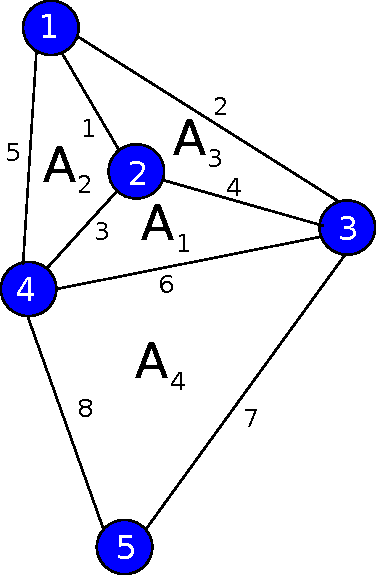
\includegraphics[scale=0.4]{Abbildungen/graph_1_planar_flach.pdf}
		\caption{Beispiel Graph (planar) mit Fl\"achen.}
	\end{center}
\end{figure}
\noindent
Die in Bemerkung 1.6. beschriebene Struktur legt ein mit planaren Graphen eng verkn\"upftes Konzept nahe. Jede Kante des Graphen ist entweder ein Bindeglied zwischen zwei Fl\"achen oder es liegt am Rand des Graphen. Die am Rand liegenden Kanten k\"onnen wiederum als Bindeglied mit der den Graphen umgebenden Fl\"ache, genannt $A_{\infty}$, angesehen werden und somit haben wir das Konzept des dualen Graphen entdeckt.
\begin{definition}
	Es sei $G$ ein planarer Graph, dann kann man einen neuen Graphen, den \textbf{dualen Graph} $G^D$, konstruieren, dessen Kanten mit denen von $G$ \"ubereinstimmen, aber dessen Ecken die Fl\"achen von $G$ zusammen mit der umgebenden Fl\"ache sind, also $V=\{A_1, A_2, \dots, A_n, A_\infty \}$. F\"ur eine gegebene Kante $e$ und Ecke des dualen Graphen $v\in V$ ist die Inzidenzmatrix Eins falls $e$ die Fl\"ache $v$ begrenzt und sonst Null.
\end{definition}
\noindent
Betrachte den dualen Graph des planaren Graphen aus Abbildung 1.5. Beachte die doppelte Kante zwischen Ecke $A_4$ und Ecke $A_\infty$. 
\begin{figure}[H]
	\begin{center}
		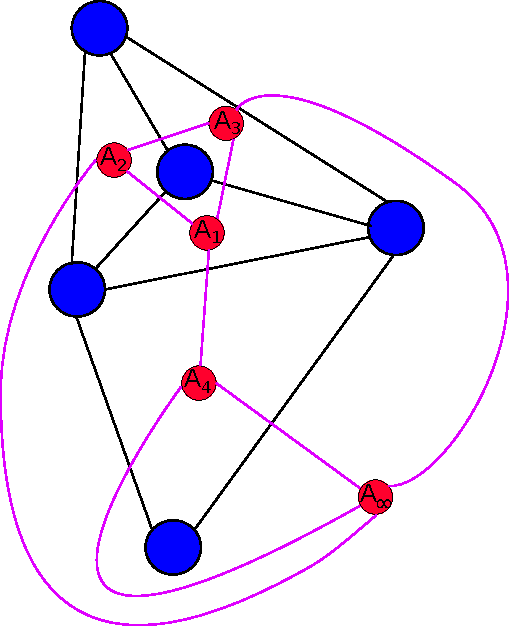
\includegraphics[scale=0.4]{Abbildungen/graph_1_dual.pdf}
		\caption{Dualer Graph des Beispielgraphen.}
	\end{center}
\end{figure}
\noindent
Die blauen Ecken symbolisieren die Ecken des Ausgangsgraphen, während die roten Ecken die Ecken des dualen Graphen darstellen. Die Platzierung von $A_\infty$ ist beliebig gew\"ahlt. Offensichtlich bestimmt diese Wahl, welcher der Ecken des Ausgangsgraphen die umgebende Fl\"ache des dualen Graphen darstellt.
\begin{remark}
	Der duale Graph $G^D$ ist immer auch fast ein planarer Graph, denn jede Ecke von $G$ kann mit einem Zyklus in $G^D$ identifiziert werden, somit bleibt aber offen welche dieser Zyklen, die umgebende Fl\"ache ist. Dies ist insbesondere von Bedeutung wenn man den dualen Graphen des dualen Graphen, den so genannten \textbf{bidualen Graphen} bildet. Um eine eindeutige Zuordnung zu erzwingen muss immer einer der Ecken ausgezeichnet werden oder man verzichtet auf die planare Darstellung und arbeitet mit Polyedern. 
\end{remark}
\noindent
Bislang wurden nur "ungerichtete Graphen" behandelt, also solche deren Kanten keine ausgzeichnete Beziehung mit der einen oder der anderen durch sie verbundenen Ecke haben. Graphen, deren Kanten eine solche Orientierung aufweisen, nennt man "gerichtete Graphen" und eine Adjazenzmatrix ist ein praktisches Weg um solche Strukturen zu beschreiben. Im Gegensatz zur Adjazenzmatrix eines ungerichteten Graphen wird im gerichteten Fall, einfach die Forderung nach Symmetrie der Matrix weggelassen.
\begin{definition}
	Jeder planare Graph kann mit einer \textbf{Orientierung} \\ausgestattet werden, dies ist eine Funktion, die jeder Kante eine der Ecken zuordnet, die durch sie verbunden wird. Man stelle sich vor jede Kante ist ein Pfeil und die Orientierung gibt an auf welche Ecke sie zeigt. Man unterscheidet entsprechend eine \textbf{Spitzefunktion} $x\mapsto p(x)$, welche die Ecke zuordnet, die an der Pfeilspitze liegt und die \textbf{Schaftfunktion} $x\mapsto q(x)$, welche die andere Ecke zuordnet.
\end{definition}
\begin{figure}[H]
	\begin{center}
		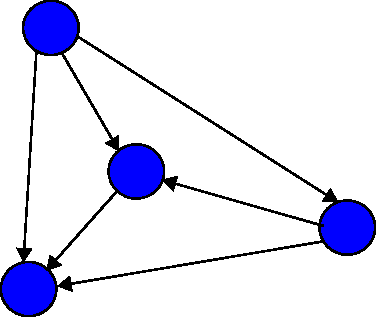
\includegraphics[scale=0.4]{Abbildungen/graph_1_orient.pdf}
		\caption{Graph mit Orientierung.}
	\end{center}
\end{figure}
\noindent
 Zu einem gegebenen Graph gibt es $2^{|E|}$ M\"oglichkeiten, wobei $E$ die Kanten\-menge ist, einen gegebenen Graph mit einer Orientierung auszustatten und ihn hierdurch zu einem gerichteten Graphen zu erheben.
 \begin{remark}
 	Jede Orientierung auf einem planaren Graph $G$, bestimmt eindeutig eine zu ihr \textbf{duale Orientierung} auf dem dualen Graph. Sei hierzu $A$ eine Fl\"ache des planaren Graphen $G$, also ein induzierter Teilgraph, der ein Zyklus ist, und $e$ eine Kante des Graphen, die auch in $A$ liegt, dann setzen wir die Spitzenfunktion $p_D$ der dualen Orientierung $p_D(e) = A$, falls $e$ im planaren Graph $G$ im Uhrzeigersinn bez\"uglich zu $A$ orientiert ist.
 \end{remark}
\begin{figure}[H]
	\begin{center}
		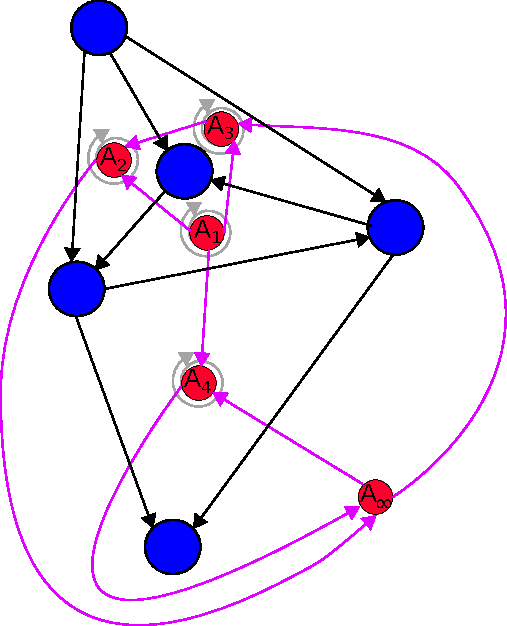
\includegraphics[scale=0.4]{Abbildungen/graph_1_dual_orient.pdf}
		\caption{Orientierung und duale Orientierung.}
	\end{center}
\end{figure}
\noindent
\chapter{Funktionenr\"aume und Operatoren}
Im letzten Kapitel wurden Graphen mit zus\"atzlicher Struktur beschrieben, nämlich planare Graphen und das Konzept des dualen Graphen. In diesem Kapitel sollen die drei Arten von Funktionen auf planaren Graphen und Operatoren, die diese Funktionen aufeinander abbilden vorgestellt werden.
\begin{definition}
	Sei $G$ ein planarer Graph und $G^D$ sein dualer Graph, des weiteren sei $V$ die Menge der Ecken, $E$ die Menge der Kanten und $A$ die Menge der Fl\"achen (inklusive umgebende Fl\"ache), dann unterscheiden wir drei verschiedene (endlichdimensionale) Funktionenr\"aume auf dieser Struktur, den Raum der Kantenfunktionen $\mathfrak{K}=\{f|f: E\rightarrow\mathbb{R}\}$, den Raum der Eckfunktionen $\mathfrak{E}=\{f|f: V\rightarrow\mathbb{R}\}$ und den Raum der Fl\"achenfunktionen $\mathfrak{F}=\{f|f: A\rightarrow\mathbb{R}\}$.
\end{definition}
\noindent
Es gibt eine nat\"urliche Beziehung zwischen diesen drei R\"aumen. 
\begin{definition}
	Sei $G$ ein Graph, $f\in\mathfrak{E}(G)$ eine Eckfunktion auf $G$, seien weiters $p$ und $q$ die Spitzefunktion und Schaftfunktion einer Orientierung auf $G$, dann nennt man $grad(f)\in\mathfrak{K}(G)$ definiert durch 
	$$grad(f)(e) = f(p(e)) - f(q(e))$$ 
	f\"ur eine beliebige Kante $e$ den Gradienten von $f$.
\end{definition}
\begin{definition}
	Sei $G$ ein Graph, $f\in\mathfrak{K}(G)$ eine Kantenfunktion auf $G$, seien weiters $p$ und $q$ die Spitzefunktion und Schaftfunktion einer Orientierung auf $G$, dann nennt man $div(f)\in\mathfrak{E}(G)$, definiert durch: 
	$$div(f)(x) = \sum_{\acute{e}\in E, q(\acute{e})=x}f(\acute{e}) -\sum_{e\in E, p(e)=x}f(e)$$
	f\"ur eine beliebige Ecke $x$ die Divergenz von $f$.
\end{definition}
\noindent
	Der Gradient hebt eine Eckfunktion auf die Kanten, und die Divergenz eine Kantenfunktion auf die Ecken. Der Graph $G$ und der duale Graph $G_D$ haben dieselben  Kantenfunktionen, daher bildet dieser Raum eine Verbindung zwischen Gradient und Divergenz des Graphen und des dualen Graphen. Der Gradient und die Divergenz des dualen Graphen werden durch $grad_D$ respektive $div_D$ symbolisiert. Falls eine Kantenfunktion als Fluss interpretiert wird, entspricht die Divergenz der Kantenfunktion dem Nettofluss von den Ecken weg.
\begin{proposition}
		Sei $G$ ein planarer Graph mit Orientierung, dann sind der Gradient und die Divergenz lineare Operatoren und es gilt:
		$$div = -grad^T$$
		wobei sich die Adjunktion auf das Standardskalarprodukt bezieht.
\end{proposition}
\begin{proof}
Sei $u\in\mathfrak{E}(G)$ und $v\in \mathfrak{K}$, dann schreiben wir das Skalarprodukt:
$$\langle v, \text{grad}(u)\rangle_\mathfrak{K} = \sum_{x\in E} v(x) * (u(p(x) - u(q(x)))) = $$
$$\sum_{x\in E} v(x) * u(p(x)) - \sum_{x\in V} v(x) * u(q(x))=$$
$$\sum_{e\in V} u(e) * \sum_{j\in E, p(j)=e}v(j) - \sum_{e\in V} u(e) * \sum_{j\in E, q(j)=e}v(j) =$$
$$-\langle \text{div}(v), u\rangle_\mathfrak{E}$$
\end{proof}
\noindent
	Es besteht eine Analogie der hier definierten Operatoren zu den Differential\-operatoren der Vektoranalysis. Interessanterweise entspricht die duale Divergenz der Rotation. Die Analogie untermauernd kann man folgendes Theorem formulieren.
\begin{theorem}[Der de Rham Komplex]
	Die Operator $grad$, $div$, $grad_D$ und $div_D$ erf\"ullen folgende exakte Sequenzen, daher das Bild der Abbildungen entspricht dem Kern der nachfolgenden Abbildung. Beachte, dass $\mathbb{R}$ in den Formeln f\"ur die dem entsprechenden Raum zugeh\"origen konstanten Funktionen steht.
\begin{equation}
	\mathbb{R}\longrightarrow\mathfrak{E}(G) \overset{grad}{\longrightarrow}\mathfrak{K}(G) \overset{div_D}{\longrightarrow}\mathfrak{A}(G)/\mathbb{R}\longrightarrow 0
\end{equation}
\begin{equation}
	\mathbb{R}\longrightarrow\mathfrak{A}(G) \overset{grad_D}{\longrightarrow}\mathfrak{K}(G) \overset{div}{\longrightarrow}\mathfrak{E}(G)/\mathbb{R}\longrightarrow 0
\end{equation}
\end{theorem}
\begin{proof}
	Wird im Kapitel "Das Poisson Problem" nachgeholt".
\end{proof}
\chapter{Das Poisson Problem}
Ein klassisches Problem der Theorie elektrischer Netzwerke sowie der Elektrostatik ist das (verallgemeinerte) Poissonproblem. Dieses Problem wird hier in einigen seiner Facetten vorgestellt und basierend auf der bisher behandelten Graphentheorie formuliert und gel\"ost.
\paragraph{Das verallgemeinerte Poisson Problem}
Sei $G$ ein planarer Graph, $\partial$ eine Teilmenge der Ecken, $r$ eine positive Kantenfunktion und $f$ und $g$ Eckfunktionen, dann wird eine Eckfunktion $u$ gesucht sodass gilt:

\begin{align}
	-div(r * grad(u))(x) = f(x)\text{  falls } x\notin \partial\\
	u(x) = g(x)\text{  falls } x\in \partial
\end{align}
Die Bedingung 2.4 ist motiviert durch Randwertprobleme aus der Theorie der partiellen Differential\-gleichungen.
\begin{definition}
	Sei $G$ ein planarer Graph mit Orientierung, $r$ eine positive Kantenfunktion, dann nennt man $\Delta_r$, definiert durch 
	$$\Delta_r(u) = -div(r * grad(u))\text{ falls }u\in\mathfrak{K}(G)$$
	den \textbf{$r$-gewichteten Laplace} Operator
\end{definition}
\paragraph{Die Formulierung f\"ur elektrische Netzwerke}Gegeben ein Netzwerk(Graph) bestehend aus Spannungsquellen, Stromquellen und linearen Komponenten (elektrische Widerst\"ande), finde  die elektrische Spannung zwischen beliebigen zwei Punkten im Netzwerk, und f\"ur jeden Leiter im Netzwerk, den durch\-flie\ss{}enden elektrischen Strom.
\begin{figure}[H]
	\begin{center}
		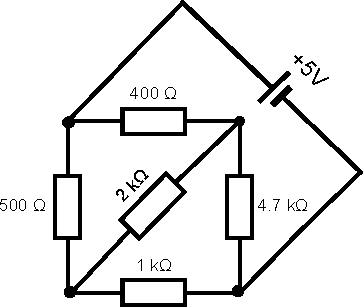
\includegraphics[scale=0.6]{Abbildungen/stromkreis_1.pdf}
		\caption{Beispiel Stromkreis.}
	\end{center}
\end{figure}
\noindent
\paragraph{Die Formulierung in der Elektrostatik} Sei $\Omega$ eine offene Teilmenge des $\mathbb{R}^3$ mit glatten Rand $\partial\Omega$ und $\rho$ die elektrische Ladungsdichte in $\Omega$. Gesucht ist das Potential $\phi:\Omega\rightarrow\mathbb{R}$ sodass:
\begin{align}
\Delta u(x) = \rho(x)\text{  falls } x\in \Omega\\
u(x) = 0\text{  falls } x\in \partial\Omega
\end{align}
Physikalisch wird $\Omega$ ein Hohlraum in einem guten elektrischen Leiter, wie etwa einem Metall, sein,  da ein Solcher das Potential am Rand des Hohlraumes auf einen konstanten Wert zwingt.\\
\\
Die Elektrostatik lebt im $\mathbb{R}^3$, daher ist die bisher entwickelte Theorie nur in Grenzf\"allen anwendbar. Dieser Spezialfall tritt ein falls $\rho$ und $\Omega$ o.B.d.A entlang der z-Achse konstant sind, daher das Problem effektiv zwei Dimensional wird. F\"ur genau diesen Fall wird eine Theorie der zweidimensionalen Maxwell Gleichungen im n\"achsten Kapitel entwickelt. 
\begin{proposition}
	Sei $G$ ein planarer Graph, $r$ eine positive Kantenfunktion und $\Delta_r$ der $r$-gewichtete Laplace Operator, dann gilt:
	\begin{itemize}
		\item Die Form der Matrix $\Delta_r$ is unabh\"angig von der gew\"ahlten Orientierung auf $G$. 
		\item $\Delta_r$ ist symmetrisch.\\
		\item $\Delta_r$ ist positiv semidefinit.\\
		\item Der Kern von $\Delta_r$ ist der Raum der konstanten Eckfunktionen.
	\end{itemize}
\end{proposition}
\begin{proof}
	Seien $p_0$ und $p_1$ Orientierungen auf $G$ und $grad_0$ und $grad_1$ die zugeh\"oringen Gradienten, dann gilt:
	$$grad_0 = D * grad_1$$
	wobei $D$ eine Diagonalmatrix ist, deren Eintr\"age $\pm 1 $ sind. Wegen Satz 2.1 folgt die erste Aussage.\\
	\\
	Die zweite Aussage folgt direkt aus der Definition von $\Delta_r$ und Satz 2.1. Seien hierzu $u$ und $v\in\mathfrak{E}$, dann gilt:
	$$\langle u, \Delta_r(v)\rangle_\mathfrak{E} = \langle \sqrt{r}*\text{grad}(u), \sqrt{r}*\text{grad}(v)\rangle_\mathfrak{K}$$
	Analog zeigt man die dritte Aussage, indem man $u=v$ setzt.
	$$\langle \sqrt{r}*\text{grad}(u), \sqrt{r}*\text{grad}(u)\rangle_\mathfrak{K}\geq 0$$
	Die letzte Aussage: $u\in\text{ker}(\Delta_r)$ gilt genau dann wenn f\"ur jedes $v\in\mathfrak{E}$
	$$\langle v, \Delta_r(u)\rangle_\mathfrak{E}=0$$
	also genau dann wenn
	$$\langle \sqrt{r}*\text{grad}(u), \sqrt{r}*\text{grad}(v)\rangle_\mathfrak{K}=0$$
	Da $r>0$ gilt, ist dies equivalent zu der Aussage $u\in\text{ker}(\text{grad})$. Der Gradient ist genau dann Null wenn $u$ konstant ist, da unser Graph zusammenh\"angend ist.
\end{proof}
\begin{theorem}
	Sei $G$ ein planarer Graph, $r$ eine Kantenfunktion, $\partial$ eine Teilmenge der Ecken und $f$ sowie $g$ Eckfunktionen, dann ist das Poissonproblem genau dann l\"osbar wenn entweder $\partial$ nicht leer ist oder $f$ im orthogonalen Komplement der konstanten Funktionen ist.
\end{theorem}
\begin{proof}
	Falls $\partial$ leer ist, folgt da der Kern von $\Delta_r$ durch die konstanten Funktionen gebildet wird und weil die Abbildung symmetrisch ist, dass der Bildraum das orthogonale Komplement der konstanten Funktionen ist.\\
	\\
	Falls aber $\partial$ nicht leer ist, aber $\partial\neq V$ ist, gilt:\\
	Sei $A$ die Untermatrix die man durch streichen der zu $\partial$ geh\"orenden Zeilen und Spalten erh\"alt, und nehmen wir an, dass diese quadratische Matrix nicht invertierbar ist, daher einen nicht trivialen Kern besitzt. Sei $x$ ein Element des Kerns von $A$ das ungleich Null ist, dann k\"onnen wir ein Element $\hat{x}$ von $\mathfrak{E}$ konstruieren, sodass $\hat{x}$ an den Ecken die zu $\partial$ geh\"oren Null hat und sonst den Wert den $x$ an der Ecke hat. Es gilt dann:
	$$\Delta_r(\hat{x})|_{E-\partial} = 0$$
	und
	$$\langle \sqrt{r}\text{grad}(\hat{x}),  \sqrt{r}\text{grad}(\hat{x})\rangle = \langle \hat{x}, \Delta_r(\hat{x})\rangle = 0$$
	Damit muss aber $\hat{x}$ zum Kern von $\partial_r$ geh\"oren, also eine konstante Funktion sein und somit gleich Null sein, ein Widerspruch.\\
	\\
	Das Setzen der Randbedingung entspricht aber genau dem Streichen dieser Zeile sowie Spalten und der Konstruktion einer zugeh\"origen im allgemeinen von Null verschiedenen Inhomogenit\"at.\\
	\\
	Der Fall $\partial=V$ ist trivialerweise erf\"ullt.
\end{proof}
\noindent
Jetzt wurden alle Grundlagen gelegt um Theorem 2.4 (de Rham Komplex) zu beweisen
\begin{proof}[Beweis de Rham Komplex]
	Es gen\"ugt Gleichung 2.1 in Theorem 2.4 zu beweisen, da 2.2 durch Anwendung von 2.1 auf den dualen Graphen folgt.\\
	\\
	Zuerst muss gezeigt werden, dass die konstanten Funktionen auf den Ecken genau der Kern von $\text{grad}$ sind. Dies wurde bereits im Satz 3.1 gezeigt.\\
	\\
	Anschlie\ss{}end muss gezeigt werden, dass das Bild von $\text{grad}$ mit dem Kern von $\Delta_r$ \"ubereinstimmt. 
	Sei $a$ ein Zyklus von $G$, und $(x_i)_{i=1}^k$ die Folge der Ecken des Zyklus im Uhrzeigersinn durchgez\"ahlt und $f\in\mathfrak{E}$, dann gilt:
	$$div_D(\text{grad}(f)) = \sum_{i=1}^{k-1} (-1)^{\sigma(i)} * (-1)^{\sigma(i)} * (f(x_{(i+1) \text{ mod } k})-f(x_{i  \text{ mod } k}))$$
	$\sigma(i)$ ist $-1$ falls die Kante zwischen $x_i$ und $x_{i+1}$ im Uhrzeigersinn durchlaufen wird und $+1$ sonst.
	Da $k \text{ mod }k=0$ gilt, kommt in der Summe jeder Wert von $f$ genau einmal mit positiven und einmal mit negativen Vorzeichen vor. Daher die Summe ist gleich Null.\\
	\\
	Abschlie\ss{}end verbleibt es zu zeigen, dass die Divergenz jeden Wert im orthogonalen Komplement der konstanten Fl\"achenfunktionen annimmt, was ja bereits durch Theorem 3.2 gezeigt wurde.
\end{proof}
\noindent
Wandeln wir zur Untermauerung der theoretischen Arbeit an einem Beispiel den elektrischen Stromkreis in Abbildung 3.1 in einen Graphen in dem bisher entwickelten Formalismus um.
\begin{figure}[H]
	\begin{center}
		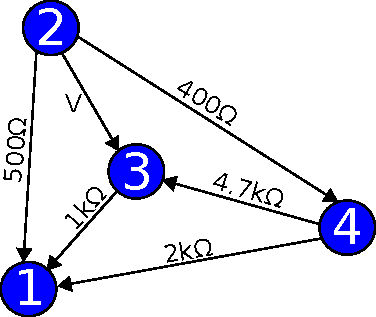
\includegraphics[scale=0.6]{Abbildungen/elektro.pdf}
		\caption{Beispiel Stromkreis (Graph).}
	\end{center}
\end{figure}
\noindent
An den elektrischen Widerst\"anden jeder Kante k\"onnen wir in Abbildung 3.2 die Korrespondenz zu Abbildung 3.1 erkennen. Die Kehrwerte der Widerst\"ande entsprechen der Kantenfunktion $r$ und $\partial=\{2, 3\}$, $g(2)=5$, $g(3)=0$ und $f\equiv 0$. Das $V$ steht f\"ur die Spannungsquelle beziehungsweise die Randbedingung.\\
\begin{center}
$
\Delta_r  = \text{grad}.T * r * \text{grad} = 
\begin{pmatrix}
1 & -1 & 0 & 0\\
1 & 0 & -1 & 0\\
1 & 0 & 0 & -1\\
0 & -1 & 1 & 0\\
0 & 0 & 1 & -1\\
0 & -1 & 0& 1\\
\end{pmatrix}^T
\begin{pmatrix}
\frac{1}{500}& 0 &0& 0& 0&0\\
0& \frac{1}{1000} & 0 & 0 &0&0\\
0 & 0 & \frac{1}{2000} & 0 &0&0\\
0 & 0 & 0 & V & 0&0\\
0 & 0 & 0 & 0 & \frac{1}{4700}&0\\
0 & 0 & 0& 0 & 0 &\frac{1}{400}\\
\end{pmatrix}
\begin{pmatrix}
1 & -1 & 0 & 0\\
1 & 0 & -1 & 0\\
1 & 0 & 0 & -1\\
0 & -1 & 1 & 0\\
0 & 0 & 1 & -1\\
0 & -1 & 0& 1\\
\end{pmatrix}=
\begin{pmatrix}
	\frac{1}{500} + \frac{1}{1000} + \frac{1}{2000}& -\frac{1}{500}  & -\frac{1}{1000} & -\frac{1}{2000}\\
	-\frac{1}{500}  & \frac{1}{500} + V + \frac{1}{400} & -V & -\frac{1}{400}\\
	-\frac{1}{1000} & -V& \frac{1}{1000} + V + \frac{1}{4700} & -\frac{1}{4700} \\
	-\frac{1}{2000} & -\frac{1}{400}&-\frac{1}{4700}  & \frac{1}{400} + \frac{1}{4700} + \frac{1}{2000}
\end{pmatrix}
$
\end{center}
Anschlie\ss{}end wendet man die Randbedingung an, daher man setzt die zweite Komponente des gesuchten Vektors $5$ und die Dritte Komponente $0$, dies entspricht dem streichen der mit $V$ markierten Ecken und bilden der passenden Inhomogenit\"at.
\begin{center}
	$
	\begin{pmatrix}[cc|c]
	\frac{1}{500} + \frac{1}{1000} + \frac{1}{2000} & -\frac{1}{2000} & \frac{5}{500}\\
	-\frac{1}{2000}& \frac{1}{400} + \frac{1}{4700} + \frac{1}{2000} & \frac{5}{400}
	\end{pmatrix}
	$
\end{center}
Dies entspricht genau der Matrixgleichung, die man mit den gebr\"auchlichen Methoden in der Physik zu diesem Problem erh\"alt.
\chapter{Die Maxwell-Gleichungen}
Die Elektrodynamik beschreibt elektromagnetische Ph\"anomene als durch Felder vermittelte Wechselwirkung von Materie. Diese Felder gehorchen vier Gleichungen, Maxwell-Gleichungen, die im neunzehnten Jahrhundert durch den Schotten James Clerk Maxwell formuliert wurden. Diese partiellen Differentialgleichungen beschreiben wie sich elektromagnetische Felder in Abh\"angigkeit eines Materiestrom zeitlich entwickeln. Die Diskretisierung jener Differentialgleichungen  f\"uhrt im zweidimensionalen Fall zu einer Variante der Maxwell-Gleichungen f\"ur planare Graphen. 
\begin{definition}
	Sei $G$ ein planarer Graph, $r$, $\epsilon$, $\sigma$, $e_0$ Kantenfunktionen, $\mu$ und $b_0$ Fl\"achenfunktionen und $q_0$ eine Eckfunktion, dann nennt man eine Schar von Kantenfunctionen $e:\mathbb{R}\rightarrow\mathfrak{K}(G)$, eine Schar von Fl\"achenfunktionen $b:\mathbb{R}\rightarrow\mathfrak{A}(G)$ und eine Schar von Eckfunktionen $q:\mathbb{R}\rightarrow\mathfrak{E}(G)$ sodass f\"ur alle $t\in\mathbb{R}$ gilt (wobei $j(t) := \sigma e(t)$)
	\begin{align}
		div(r * \epsilon * e(t)) = q(t)\\
		div_d(r * e(t)) = -\frac{\partial b(t)}{\partial t}\\
		r * grad_d(\mu * b(t)) = \epsilon * \frac{\partial e(t)}{\partial t} + j(t)
	\end{align} 
	und die Anfangsbedingungen
\begin{align}
	e(0) = e_0\\
	b(0) = b_0\\
	q(0) = q_0
\end{align}
erf\"ullt sind, eine L\"osung der Maxwell-Gleichungen.
\end{definition}

\end{document}
das poisson problem randbedingung die in zusammenhangskomponenten zerfallen lässt.
dirchlet und neumann
